\section{分裂法与全分离法}
\label{sec:2.4}
通常同时起作用的两个过程A与B也许是或者
也许不是相互联系的。它们相互独立的这种情形, 称作全分离(full separation)
。在这种情形下,就概念和就计算而言,想像A过程在B过程开始之
前正趋近于结束,这往往是很有用的。在两种过程
彼此有相互联系的场合,有可能是允许A短暂起作
用,然后转换为B起作用,并如此交替作用下去,
这种交替起作用的办法称作分裂法(splitting)。

\subsection{热流方程}
\label{sec:2.4.1}
绕射方程或偏移方程可称作“波阵面恢复”方程,它把初始条件或透镜项可能引起的波阵面的任
何横向突变一起加以平滑恢复原状。
15°偏移方程具有有与热流方程相同的数学形式。不过热
流方程全是实数,而且它的物理性态更容易理解,这点值得多说两句:(l)x方向的热流
$H_x$等于温度的负梯度$-\partial T/\partial x$如乘以热传导率$\sigma$。(2)温度降低$-\partial T/\partial t$是同热流发散量$\partial H_x/\partial x$
除以热容量c成比例。将上述二者结合起来并由一维情形推广至二维情形,取$\sigma$为常数及
$c=l$,得出方程:
\begin{equation}
\frac{\partial T}{\partial t}=\sigma[\frac{\partial^2}{\partial x^2}+\frac{\partial^2}{\partial y^2}]T
\label{eq:ex2.4.1}
\end{equation}

\subsection{分裂法}
\label{sec:2.4.2}
应用于热流方程数值解法的分裂法是用两个微分方程代替热流方程,按交替的时间步长
应用其中每个方程
\begin{subequations}
\begin{equation}
\frac{\partial T}{\partial t}=2\sigma\frac{\partial^2 T}{\partial x^2} \quad (all\quad y)
\label{eq:ex2.4.2a}
\end{equation}
\begin{equation}
\frac{\partial T}{\partial t}=2\sigma\frac{\partial^2 T}{\partial y^2} \quad (all\quad x)
\label{eq:ex2.4.2b}
\end{equation}
\label{eq:ex2.4.2}
\end{subequations}

式\ref{eq:ex2.4.2a}中,对于x方向的热流其热传导率$\sigma$业已增大两倍,而对$y$方向的热流则已取$\sigma$
为零;在式\ref{eq:ex2.4.2b}中,则情形反之。在时间的奇数时刻,热量按式\ref{eq:ex2.4.2a}的关系流
动;在时间的偶数时刻则按式\ref{eq:ex2.4.2b}的关系流动。这种轮流交替采用式\ref{eq:ex2.4.2a}与
\ref{eq:ex2.4.2b}所得的解在数学上可证明是收敛于式\ref{eq:ex2.4.1}的解,其误差为$\Delta t$数量级,因此
汾趋于零时,误差亦趋于零。高维隐式方法的不可行性是促使采用分离法的原因(参阅\ref{sec:2.2}
节结尾部分)。

\subsection{全分离法}
\label{sec:2.4.3}
最终可证明分裂法比可能想像的要精确得多,在许多情形下不存在精度损失。此外,可
认为这种方法是一种极限情形。试考虑一下处理方程\ref{eq:ex2.4.2a}与\ref{eq:ex2.4.2b}的基本方
法,在这种处理中,不是按交错的时间步长在它们之间轮流进行前向与后向计算,而是通过
所有时间步长将方程\ref{eq:ex2.4.2a}计算到底,然后再将这种中间计算结果作为方程\ref{eq:ex2.4.2b}
的初始条件,经过所有时间步长将式\ref{eq:ex2.4.2b}计算到底,得出最终结果。也许会令人惊
奇,这种经过基本改变的方法可以产生方程\ref{eq:ex2.4.1}的正确解。但是,只在$\sigma$是$x$与$y$的一个恒定
函数时,才能如此。对于脉冲型初始扰动的情形,该种过程如图\ref{fig:txz/temperature}所示。在用这种基本
方法获得正确的解时,就把像\ref{eq:ex2.4.1}那样的一种微分方程说成是可全分离的。全分离法
在$\sigma$为常数时才有效,这点不应使人感到太奇怪,因为这时才能够应用Fourier变换,从而
二维解$exp[-\sigma(k_x^2+k_y^2)t]$等于一维解$exp(-\sigma k_x^2t)$与$exp(-\sigma k_y^2t)$之乘积。可以证明
并且以后将会指出,可应用全分离法的条件就是$\sigma \partial^2/\partial x^2$应能与$\sigma \partial^2/\partial y^2$交换。从技术上说,
还存在一个边界条件的要求,不过当扰动在到达边界之前即衰减掉时,这点不会造成什么困
难。
\begin{figure}[H]
\centering
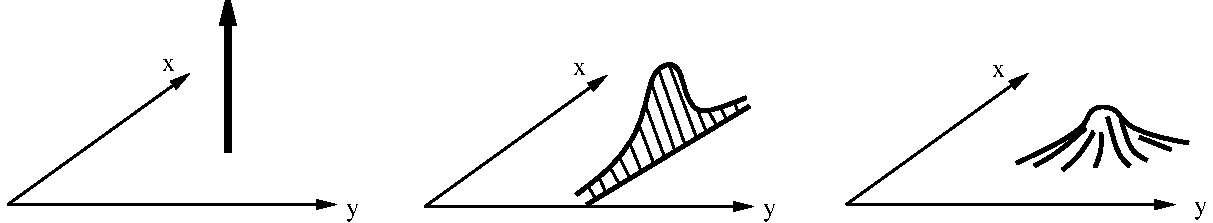
\includegraphics[width=0.95\textwidth]{txz/temperature}
\caption[temperature]{$(x,y)$平面内的温度分布。开始时为delta函数形状(左)。允许沿$x$方向但不沿$y$方向流动之后,热
量分希位于一片状区域内(中)。最后,允许热量沿$y$方向但不沿$x$方向流动,
得出同样的对称高斯分布的结果,其最终形状犹如热量同时沿$x$方向与$y$方向
流动,(右)}
\label{fig:txz/temperature}
\end{figure}


令人奇怪,在许多有关数值解的教科书中对全分离性没怎么介绍,这也许是由于不论是用
分裂法还是用全分离法求解,其加法与乘法的总次数是相同之故。但是,作为一个实际问
题,求解大数据量问题的计算时间并非简单随乘法次数而增高。当数据库不能整个输入于随
机存取器时(这差不多就是大数据量问题的定义),则分裂法的每一步骤都要求将数据库
加以转置。例如,从$(x,y)$的存储顺序转置成$(y,x)$的存储顺序。转置所要求的就不
是乘法,可是在许多情况下,转置所需时间却远超出整个计算所耗费的时间。所以,若进行
转置是不能避免时,至少应使它减少至实际允许的极小限度。有一些情况使得非在分裂法与
全分离法之间采取折中办法不可。例如,如果$\sigma$是$x$与$y$的一个缓慢变化的函数
时,就得如此,这时会发现,虽然$\sigma \partial^2/\partial x^2$并非严格可与
$\sigma \partial^2/\partial y^2$交换,可是却足够接近,因而在对数据进行转置
和转换至式\ref{eq:ex2.4.2b}之前,能够继续用式\ref{eq:ex2.4.2a}进行若干时间
步长的计算。以下要考虑的波场外推方程就是类似于这样一种但更具有地球物理意义的情况。第一个认识
到分裂法与全分离法概念在地震学中的意义是Brown(1983)。

\subsection{应用于横向速度变化情形}
\label{sec:2.4.4}
有一种情况:其中两个微分算子的不可交换性程度具有简单物理意义,且有明显有效之
地球物理应用,这种情形就是适用于非均匀介质的所谓单频15°波场外推方程。取时,
这种方程为
\begin{equation}
\frac{\partial U}{\partial z}=\{\frac{i\omega}{\bar{v}(z)}+i\omega
[\frac{1}{v(x,z)}-\frac{1}{\bar{v}(z)}]-\frac{\bar{v}(z)}{2i\omega}
\frac{\partial^2}{\partial x^2}\}U\\
=(retardation\quad + \quad thin\quad lens\quad +\quad diffraction)U
\label{eq:ex2.4.3}
\end{equation}
由式\ref{eq:ex2.4.3}可知,延迟项与薄透镜项可交换,且与自由空间绕射项可交换,但薄透镜项
与绕射项却彼此不能交换。看来,实际上最好是采用分裂法,用解析方法处理薄透镜项而用
Crank-Nicolson方法处理绕射项,这时,稳定性是有保证的,因为单独各个问题的稳定性
均已知。还有,解析解的精度也是引人入胜的一种特点。现在的问题是,这样两项在什么程
度上是可交换的?

这问题正好是幻灯投影仪的聚焦问题,调节聚焦旋钮就相当于调整薄透镜项,使之可与
自由空间绕射项相比。有的是小范围微调,没一个人能察觉出有任何差别;有的是大范围调
节,使后排座位的人不受错误聚焦的干扰。许多地球物理数据处理就是向下延拓数据,出现
在透镜项中的速度横向变化仅可已知到有限精度,要应用它就得利用外推办法来确定
$v(x)$。

对于很长的横向空间波长,各项是互换的,这时可忽略速度$v$之横向变动而进行绕射项
处理。波长较短时,则绕射项影响与透镜项影响必然是兼而有之。所以,现实问题并非仅仅
是计算的方便与不方便,而是数据精度与地下模型内速度可能变化范围之间的相互影响问题。

\subparagraph{应用于三維向下延拓}
\label{sec:2.4.5}

三维零炮检距反射地震资料的偏移算子是可利用Taylor级数展开至二阶的、即展开为
所谓的15°近似
\begin{equation}
[\frac{(-i\omega)^2}{v^2}-\frac{\partial^2}{\partial x^2}-\frac{\partial^2}{\partial y^2}]^{1/2}
\approx -\frac{i\omega}{v}-\frac{v}{-2i\omega}\frac{\partial^2}{\partial x^2}-\frac{v}{-2i\omega}\frac{\partial^2}{\partial y^2}
\label{eq:ex2.4.4}
\end{equation}
